\chapter{Datenspeicherung}
\label{ch:data_persistence}

\section{Allgemeiner forensischer Analyseprozess}
Im Praxisteil dieser Arbeit soll eine Analyseplattform auf Basis von Apache Hadoop aufgebaut werden. Diese Analyseplattform dient zur Auswertung sichergestellter Beweismittel und dem Auffinden von Beweisen in großen Datenmengen. Hierbei behandelt die Analyseplattform aber nur einen Teil der Arbeitsvorgänge während einem forensischen Analyseprozess.\\

\noindent
Abbildung \ref{fig:digital_forensics_process} skizziert einen allgemeinen forensischen Analyseprozess für digitale Beweismittel.\cite[S.16]{digital_forensics} Die grün hinterlegten Schritte definieren den Arbeitsbereich, bei welchen die hier entwickelte forensische Analyseplattform den Forensiker unterstützen kann.\\ 
\begin{figure}[ht]
  \centering
  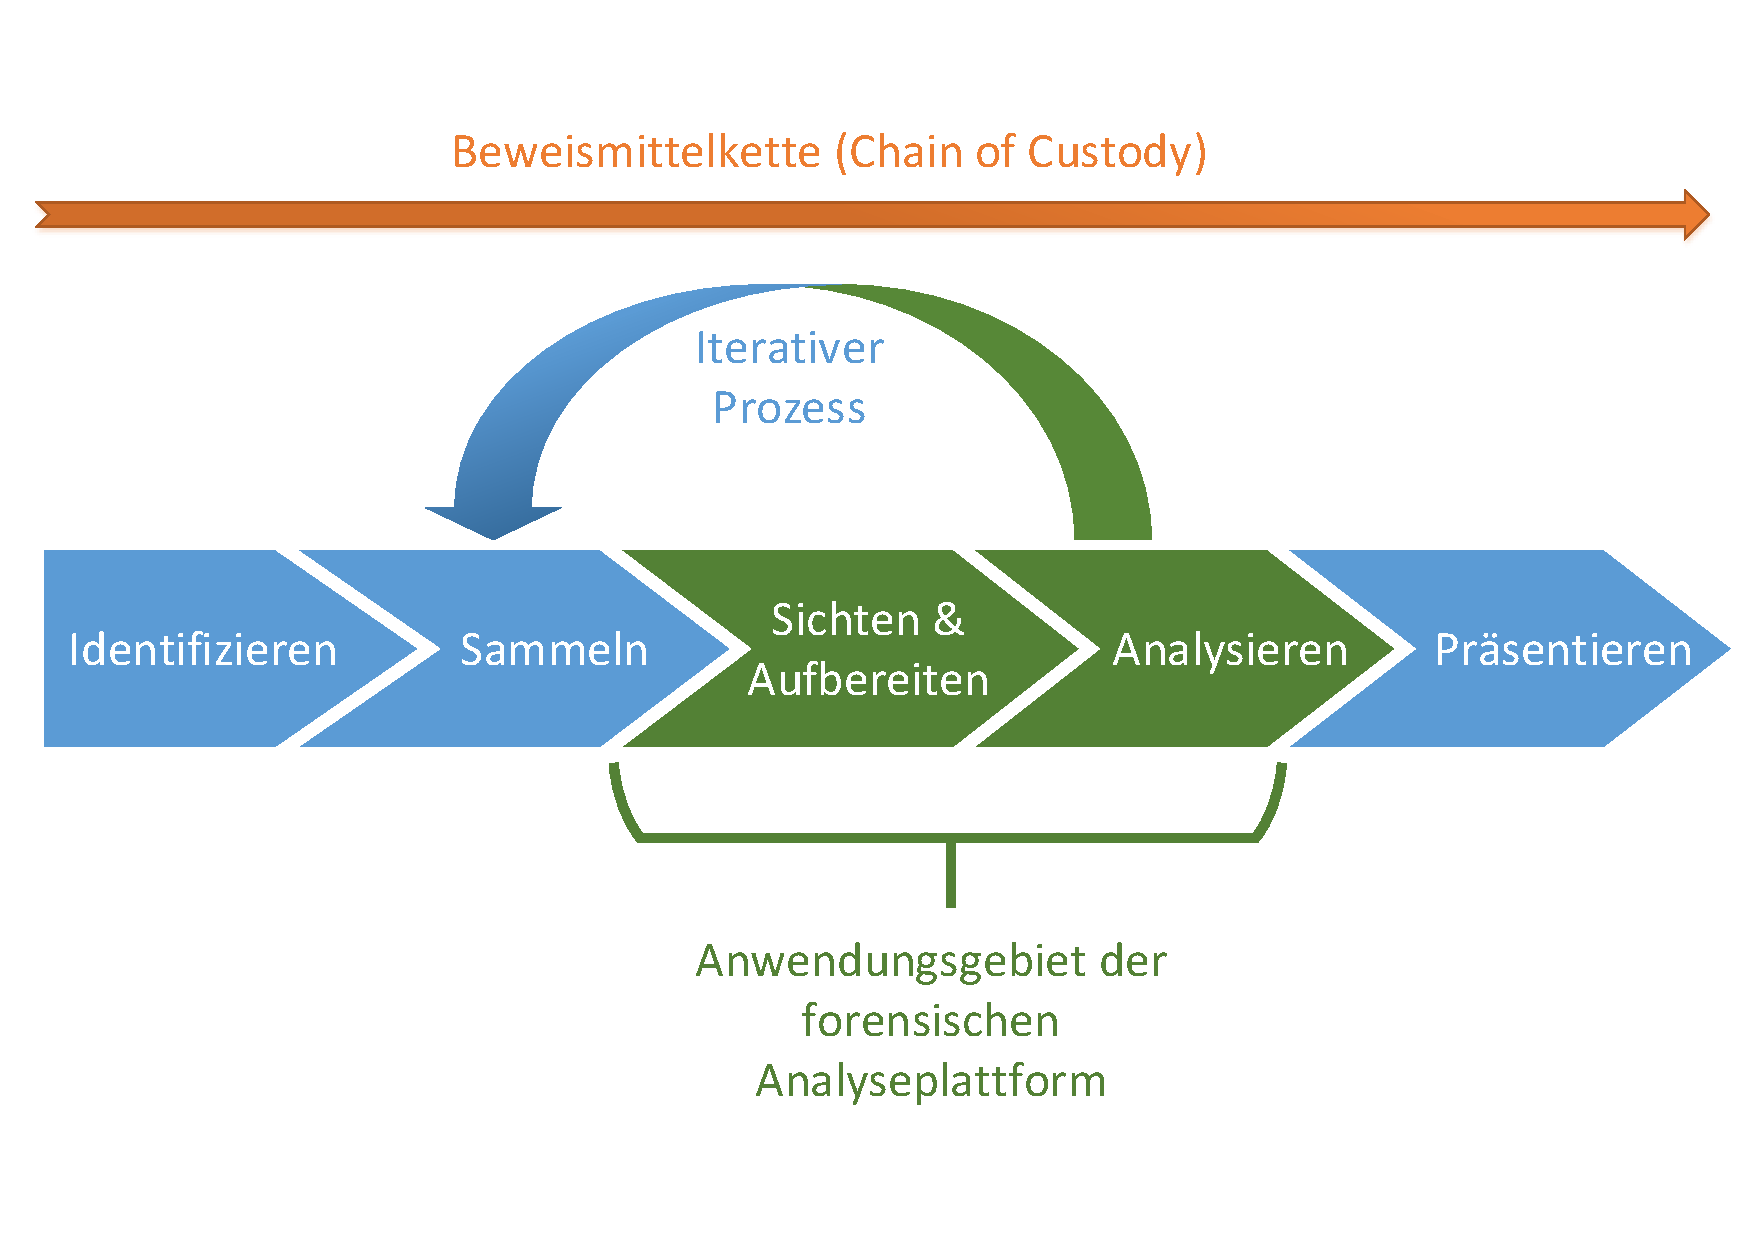
\includegraphics[width=\textwidth]{./resource/digital_forensics_process.pdf}
  \caption{Forensischer Analyseprozess für digitale Beweismittel (Vgl. \cite[S.16]{digital_forensics})}
  \label{fig:digital_forensics_process}
\end{figure}


\noindent
Zu Beginn existiert ein Vorfall oder ein Tatverdacht für eine Straftat. In einem nachfolgenden Schritt ermittelt beispielsweise die Staatsanwaltschaft. Im Ermittlungsverlauf wird darauf der Tatort untersucht oder auch bei Tatverdächtigen nach Hinweisen für die Tat und gegebenenfalls deren Tathergang gesucht. Dieser Schritt beschreibt die Identifikationsphase aus Abbildung \ref{fig:digital_forensics_process}. Hierbei geht es um die Identifikation von möglichen Beweismittel, welche sichergestellt oder  beschlagnahmt werden sollen.\cite[S. 17-24]{digital_forensics}.\\ In der Forensik wird häufig hypothesenbasiert vorgegangen. So entwickelt der Ermittler eine Hypothese, wie eine möglich Straftat begangen wurde und wer diese begangen haben könnte. Darauf aufbauend überlegt er sich welche Spuren für oder gegen diese Hypthese sprechen und welche möglichen Beweismittel eben diese Spuren enthalten könnten (z.B. Kommunikationsdaten auf dem PC oder Bildmaterial auf einem Mobiltelefon).\\

\noindent
Im zweiten Schritt aus Abbildung \ref{fig:digital_forensics_process} geht es um das Vereinnahmen von potentiellen Beweismitteln. Hierbei werden dann die identifizierten Datenträger und Geräte sichergestellt oder beschlagnahmt. In dieser Phase werden beispielsweise auch schon forensisch korrekte Datenträgerabbilder erstellt, auf welchen dann später eine Datenanalyse ausgeführt werden kann.\cite[S. 24-33]{digital_forensics}. In vielen Fällen, beispielsweise bei Unternehmensservern, werden nicht die Geräte selbst sichergestellt sondern nur wichtige Daten forensisch korrekt kopiert. Auch hier findet teilweise schon eine Vorselektion statt, welche Daten benötigt werden und welche Daten im konkreten Fall irrelevant sind.\\

\noindent
Die dritte Phase aus Abbildung \ref{fig:digital_forensics_process} behandelt das Sichten und Aufbereiten der sichergestellten Daten. Gerade bei großen unstrukturierten Datenmengen erfolgt in dieser Phase auch eine Vorselektion, um die Datenmenge nochmals einzugrenzen. Dies kann automatisiert oder auch manuell erfolgen.\cite[S. 33-39]{digital_forensics}. An dieser Stelle beginnt das Anwendungsgebiet der hier entwickelten forensische Analyseplattform. 
So können alle gesammelten Daten in die forensische Analyseplattform importiert und prozessiert werden. Darauf kann über eine allgemeine Suche nach spezifischen Stichworten, Hashsummen oder Zeitpunkten gesucht werden. Dies soll dem Ermittler das Auffinden von fallreleventen Daten erleichtern. Die meisten bekannten forensischen Analysetools bieten ebenfalls Stichwortsuche an, weil eben dadurch große Datenmengen schnell nach bestimmten Kriterien gefiltert werden können.\cite[S. 116-123]{handbook_digital_forensics}\\
In dieser Phase werden aber auch gelöschte, verschlüsselte oder verschleierte Daten wiederhergestellt oder entschlüsselt, sofern dies möglich ist. Eine klassische Methode ist beispielsweise auch das sogenannte \textit{File Carving} auf Datenträgern.\cite[S. 38-39]{digital_forensics}\footnote{Beim File Carving wird versucht logisch zusammenhängende Daten allein anhand des Dateiinhalts zu rekonstruieren, ohne die Dateisystemmetadaten zu nutzen. Die Methode wird gerne angewendet, wenn das Dateisystem nicht wiederherstellbar ist oder wenn gelöschte Dateien auf bereits freigegebenen Speicherbereichen gesucht werden.} Diese Art von Datenaufbereitung beherrscht die hier entwickelte forensische Analyseplattform derzeit noch nicht.\footnote{Es wäre aber durchaus möglich diverse Methoden der Datenaufbereitung zu implementierten. Siehe auch Kapitel \ref{ch:ausblick}.}\\

\noindent
Auch in der anschließenden Analysephase kann die hier entwickelte forensische Analyseplattform genutzt werden (siehe Abbildung \ref{fig:digital_forensics_process}). In dieser Phase werden die aufbereiteten Daten detailliert analysiert, um Informationen zu erhalten die für oder gegen einen bestimmten Tathergang sprechen.\cite[S. 39-45]{digital_forensics} Anhand dieser Informationen werden die eingangs beschriebenen Hypothesen zu möglichen Tathergängen verifiziert. Bei einer Analyse werden aus den Daten komplexe Zusammenhänge und Beziehungen erarbeitet. Beispielsweise werden aus den Rohdaten Kommunikationsverläufe auf Basis von E-Mails oder zeitliche Abläufe basierend auf Zeitstempelanalysen erstellt.\cite[S. 33-39]{digital_forensics}\\
Hierbei geht es auch darum die Aussagekraft eines potentiellen Beweismittels zu ermitteln. So könnte beispielsweise urheberrechtsverletzendes Material auf einem Datenträger eines PCs gefunden werden. Allerdings kann die Aussagekraft dieses potentiellen Beweismittels sehr gering sein, wenn das System bereits durch Schadsoftware kompromittiert wurde.\\
Einige Analyseschritte können automatisiert werden und sind daher prädestiniert für die hier entwickelt Analyseplattform (siehe auch Kapitel \ref{ch:data_processing}).\\

\noindent
Bei der Analyse können auch wieder Verbindungen zu neuen potentiellen Beweismitteln gefunden werden, welchen dann wieder über den forensischen Analyseprozess vereinnahmt und aufbereitet werden. Daher ist der Prozess auch iterativ anzusehen. Gerade durch die Nutzung der forensischen Analyseplattform sollen diese Iterationen verkürzt werden, indem durch die parallelisierte Prozessierung Zeit eingespart werden soll.\\

\noindent
In der letzten Phase des Analyseprozesses müssen die Ermittlungsergebnisse visuell aufbereitet werden, um sie auch vor Gericht präsentieren zu können. Letztlich muss ein Analysebericht erstellt werden, welcher einerseits die Ergebnisse enthält und andererseits nachvollziehbar beschreibt, wie diese Analyseergebnisse zustande gekommen sind.\footnote{Der Bericht sollte so geschrieben sein, dass andere Parteien oder Ermittler die gleichen Ergebnisse reproduzieren können.}\cite[S. 45-47]{digital_forensics}. Viele Analysetools, unter anderem auch das hier genutzt Referenztool \textit{Autopsy}, ermöglichen die semi-automatische Erstellung von Analyseberichten. Die hier entwickelte Analyseplattform kann dies derzeit noch nicht. Bei einer Weiterentwicklung der Analyseplattform wäre diese Funktionalität aber durchaus brauchbar.\\

\noindent
Ein primärer Aspekt bei dem allgemeinen forensischen Analyseprozess aus Abbildung \ref{fig:digital_forensics_process} ist letztlich die Dokumentation der Beweismittelkette. Mit ihr steht und fällt die Aussagekraft der Ergebnisse aus einer forensischen Analyse.\footnote{In der Vergangenheit gab es immer wieder Fälle, bei welchen eine fehlerhaft dokumentierte Beweismittelkette zu sehr fragwürdigen Aussagen auch bei ursprünglich eindeutigen Beweislagen führte.} Daher muss bei der Dokumentation der Beweismittel lückenlos festgehalten werden, was mit letzteren passiert ist. Nachfolgende Liste lieferte hierzu wichtige Kriterien, die festgehalten werden müssen:
\begin{itemize}
\item Die Ermittler, welche das Beweismittel sichergestellt und später analysiert haben.
\item Die Prozesse, Datenaufbereitungen und Analysen, welche durchgeführt wurden.
\item Die Zeitpunkte der Sicherstellung, Aufbereitung und der Analyse.
\item Die Umstände, wie das Beweismittel sichergestellt wurde.
\item Gründe, wieso das Beweismittel sichergestellt wurde.
\item Transportwege und Lagerstätten der Beweismittel.
\item Personen die Zugang zu den Beweismittel hatten und allgemeine Informationen, wie die Beweismittel vor unbefugten Zugriff geschützt wurden.
\end{itemize}

Ein sehr wichtiger Punkt bei der Dokumentation der Beweismittelkette ist Verifikation der Datenintegrität des Beweismittels während des gesamten Analyseprozesses. Dies wird primär durch die Prüfung mittels kryptografischer Hashes erreicht. Letztlich dienen diese zum Schutz vor einer unbeabsichtigten oder beabsichtigten Modifikation des Beweismittels. Das Ändern von Beweismittel oder deren Kopien sollte eigentlich immer vermieden werden. In vielen Fällen ist dies jedoch notwendig, um beispielsweise defekte Datenstrukturen wiederherstellen zu können. Bei solchen bewussten Datenänderungen ist eine entsprechende Dokumentation notwendig.\\ 
Bei der Analyse mit der hier entwickelten Analyseplattform muss auch die Beweismittelkette entsprechend dokumentiert werden. Diese Thematik wird im Rahmen dieser Thesis zumindest in der Theorie nochmals diskutiert. Die derzeitige Implementierung der forensischen Analyseplattform behandelt diesen Aspekt derzeit noch nicht. Aber auch hier könnte in einer Weiterentwicklung eine Beweismittelkette erstellt werden, welche die einzelnen Verarbeitungsprozesse, Zeitpunkte und Nutzerzugriffe dokumentiert.\\



\section{Herkömmliches Analysevorgehen}
\label{sec:common_analysis_approach_part1}
Um die fachlichen Anforderungen an das Analyse-System herauszuarbeiten, soll das herkömmliche Analysevorgehen mit einem vergleichbaren Open-Source Analysewerkzeug betrachtet werden.\\
Die Ausgangslage liefern einige Datenträgerabbilder aus diversen Testszenarien. Diese Datenträgerabbilder sind bezogen auf den forensischen Analyseprozess aus Abbildung \ref{fig:digital_forensics_process} die Grundlage für dir dritte Phase - dem Sichten und Aufbereiten der Daten.

\noindent
Bei gängigen Analysevorgehen werden beispielsweise die Datenträgerkopien mit Betriebssystemprogrammen unter Linux oder mithilfe des Open-Source Analysetools \textit{Autopsy}\footnote{Siehe \url{https://www.sleuthkit.org/autopsy/}. Hierbei wird die Version 4.7.0 in der 64-bit Variante unter Windows 10 Pro genutzt.} unter Windows analysiert. Im kommerziellen Bereich existieren etliche weitere Analyse-Tools mit größerem Funktionsumfang. Nachfolgend wird Autopsy als Referenzsystem unter Windows betrachtet, da es eines der bekanntesten Analysewerkzeuge unter den kostenfreien Open-Source Programmen ist. \\ 

\noindent
Die Datenträgerabbilder können in unterschiedlichen Dateiformaten vorliegen. Mithilfe klassischer Opensource-Tools wie beispielsweise \textit{dd}\footnote{dd ist ein bekanntes Werkzeug zum Kopieren von Daten, welches unter den meisten Unix-basierten Betriebssystemen läuft. Damit können auch ganze Partitionen in einzelne logische Dateien kopiert werden.} kann damit ein Image im sogenannten \textit{RAW}-Format erstellt werden. Von \textit{dd} existiert auch eine forensische Variante \textit{dcfldd} welche beim Kopieren auch noch Hashsummen zur Verifikation berechnet.\cite{linux_forensics}  Andere Tools, wie beispielsweise \textit{FTK-Imager} können auch Datenträgerabbilder in speziellen Container-Formaten erstellen und lesen. Beispielsweise gibt es das \textit{EnCase Physical}-Format mit der Dateiendung \textit{.e01}, oder das \textit{Advanced Forensic Format} mit der Endung \textit{.aff}.\footnote{Siehe \url{https://support.accessdata.com/hc/en-us/articles/222778608-What-Image-Formats-Do-AccessData-Products-Support-}, Stand: 4.4.2018.} Diese Formate unterstützen eine bessere Extraktion von Metadaten oder bieten eine zusätzliche Datenkompression oder Verschlüsselung der darin gespeicherten Dateien an.\cite[S. 35]{digital_forensics}\\

\noindent
Es wird auch unterschieden, ob es sich um ein vollständiges Datenträgerabbild handelt oder um ein logisches Dateiarchiv. Bei dem vollständigen Datenträgerabbilder werden auch nicht allokierte Speicherbereiche innerhalb des Dateisystems, der Partition oder des Datenträgers gesichert. Hier können sich potentiell versteckte und gelöschte Dateifragmente befinden. Auf diesen Datenträgerabbilder kann auch das bereits beschriebene File Carving ausgeführt werden, um gelöschte Dateien wiederherzustellen.\\ 
Ein logisches Dateiarchiv hingegen enthält wirklich nur die Dateien auf einer logischen Ebene und keine unallokierten Speicherbereiche. Von Vorteil hierbei ist eine geringere Speichergröße. Allerdings tritt durch die logische Sicherung ein potentieller Informationsverlust auf, da unallokierte Speicherbereiche nicht berücksichtigt werden, die aber dennoch potentiell auswertbare Informationen liefern könnten. Vertreter logischer Darteiarchive sind die allseits bekannten Archiv-Formate wie beispielsweise ZIP oder TAR.\\

\noindent
Letztlich werden die Beweismittel in unterschiedlichsten Formaten auf dem lokalen Analyse-Rechner gespeichert. Darauf aufbauend können die Daten in spezifische Formate konvertiert werden. Dies hängt aber meistens davon ab, wie sie weiter verarbeitet werden sollen und welche Werkzeuge zu dieser Verarbeitung genutzt werden.\\

\noindent
Im konkreten Testszenario ist das Datenträger-Abbild eines Linux-Rechners im RAW-Format auf dem lokalen Analyse-Rechner gespeichert. Das Abbild selbst kann ein oder mehrere Partitionen enthalten. Innerhalb der Partition werden Daten mithilfe unterschiedlicher Dateisysteme strukturiert gespeichert. Diese Dateisysteme können unter Windows mit dem Werkzeug \textit{X-Mount} oder unter Linux direkt mit dem Befehl \textit{mount} schreibgeschützt gemountet werden. Darauf wird das Dateisystem vom Betriebssystem interpretiert und als logisches Volume auf dem Analyse-Rechner bereitgestellt. Nun können die Dateien mit beliebigen Werkzeugen analysiert werden.\\

\noindent
In der Praxis hat das einfache schreibgeschützte Mounten den Vorteil, dass der Analyst relativ schnell im Dateisystem beliebige Dateien finden und dessen Inhalt mit diversen Tools anzeigen kann. Gerade für eine schnelle Vorprüfung ist dies sinnvoll. Im nachfolgenden Kapitel sollen nun Möglichkeiten zur Speicherung und Aufbereitung des Datenträgerabbildes mithilfe der forensischen Analyse-Plattform untersucht werden.\\

\noindent
Nachfolgend wird nun gezeigt wie ein Datenträgerabbild in einem konkreten Beispiel mit Autopsy (Version 4.7.0 64-bit) unter Windows 10 geöffnet und analysiert wird.\\
Zu Beginn wird bei Autopsy ein neuer Fall erstellt. Hierbei kann ein Name für den Fall angegeben werden und ein Verzeichnis, worin Autopsy die Anwendungsdaten der Analyse speichert. Danach können noch einige optionale Informationen, wie beispielsweise der Bearbeiter, Adressdaten, die Organisation und eine kurze Beschreibung angegeben werden (siehe Abbildung \ref{fig:autopsy_1_case_information}). Bei der Erstellung des Falles wird unter anderem eine neue Falldatenbank angelegt. Diese Datenbanken werden alle lokal auf dem Analyserechner gespeichert.\\

\begin{figure}[ht]
  \centering
  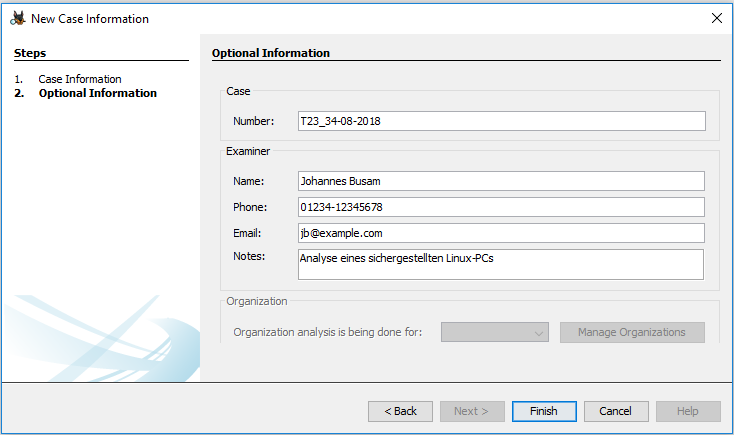
\includegraphics[width=\textwidth]{./resource/autopsy_1_case_information.png}
  \caption{Erstellung eines neuen Falles mit Autopsy}
  \label{fig:autopsy_1_case_information}
\end{figure}

\noindent
Im nächsten Schritt kann nun eine neue Datenquelle dem Fall hinzugefügt werden. Es werden folgende Typen von Datenquellen unterstützt:
\begin{itemize}
\item Ein Datenträgerabbild im \textit{RAW-Format}-Format, Encase-Format oder ein Abbild einer virtuellen Maschine (z.B. von Virtual Box).
\item Ein lokales Laufwerk (z.B. eine externe Festplatte).
\item Logische Dateien aus einem verfügbaren Dateisystem (z.B. ein beliebiger Ordner).
\item Ein Abbild eines beliebigen Speicherbereiches in einer Datei.
\end{itemize}

\noindent
Im konkreten Fall wird ein Datenträgerabbild als Datenquelle hinzugefügt. Dabei muss auch noch eine Zeitzone angegeben werden. Diese Zeitzone kann entscheidend für die Analyse der Zeitstempel auf einem Datenträger sein. In einem \textit{ext}-Dateisystem bei gängigen Linux-PCs werden die Zeitstempel als Anzahl der Sekunden seit dem 1. Januar 1970 in der Zeitzone UTC gerechnet.\cite[S. 326]{filesystem_forensic}\footnote{Diese Zeitdefinition entspricht der sogenannten Unixzeit.} Bei den älteren \textit{FAT}-Dateisystemen hingegen wird die Zeit ohne Zeitzone gespeichert.\cite[S. 192-194]{filesystem_forensic} Je nachdem in welcher Zeitzone das Betriebssystem konfiguriert wurde, welches die Dateien in dem FAT-Dateisystem änderte, ergeben sich zeitliche Unterschiede. Daher muss bei Zeitstempeln auch später bei der Anzeige der Analyseergebnisse immer auch auf die Zeitzone geachtet werden.\footnote{Ein weiteres interessantes Problem ergibt sich auch bei der Sicherung der Beweismittel an einem Tatort. Auch dort ist nie garantiert, dass alle gesicherten Beweismittel überhaupt zeitlich synchronisiert sind. Gerade in Kombination mit Netzwerkverbindungsdaten können bei einer fehlenden Zeitsynchronisation kritische Abläufe zeitlich versetzt sein. Daher muss gerade die Aussagekraft von Zeitstempel immer kritisch betrachtet werden.}\\

\noindent
Im nächsten Schritt können diverse Module zur Datenaufbereitung aktiviert werden. Diese Module dienen zur automatischen Datenaufbereitung und werden ausführlich in Kapitel \ref{sec:common_analysis_approach_part2} beschrieben. In dem Kapitel erfolgt dann auch der Vergleich zur der automatisierten Auswertung mit der hier entwickelten Analyseplattform.\\
Nachdem die entsprechende Module ausgewählt wurden, beginnt Autopsy die Datenquelle zu analysieren. Dies läuft vollständig im Hintergrund ab und der Nutzer kann parallel hierzu die Datenquelle manuell analysieren.\\ 

\noindent
Das Importieren einer Datenquelle bei Autopsy besteht letztlich aus dem Erstellen eines Falls und der Angabe einiger Konfigurationsmöglichkeiten. Die eigentliche Datenquelle wird hierbei nicht in einen internen Anwendungsordner kopiert sondern wird während der Analyse auf dem Rechner bereitgestellt (entweder als Datenträgerabbild oder direkt als externer Datenträger). In den Anwendungsordner selbst werden Metainformationen, wie beispielsweise die Indexierung bestimmter Daten, abgespeichert um während der Analyse schneller darauf zugreifen zu können. Prinzipiell ist dieses Vorgehen sehr gut, da der Ermittler direkt mit der Arbeit beginnen kann und keine Daten mehr kopieren muss.\footnote{Das Erstellen eines Datenträgerabbildes aus dem originalen Asservat wurde hierbei schon vorher durchgeführt.}

\section{Umsetzung in der Hadoop Analyse-Plattform}

Im vorangegangen Kapitel wurde bereits beschrieben, wie bei Autopsy Datenträgerabbilder als sogenannte Datenquellen in die Analysesoftware importiert werden. Wie erwähnt wird das Datenträgerabbild oder der extern angeschlossene Datenträger nicht in einen internen Anwendungsordner kopiert. Autopsy arbeitet direkt auf den Daten um ein unnötiges Kopieren von Daten und dessen Ressourcenaufwand zu vermeiden. \\

\noindent
Im Vergleich hierzu arbeitet die hier entwickelte forensische Analyseplattform auf einem eigenen Computer-Cluster basierend auf mehreren Knoten und nicht nur auf einem einzelnen Analyserechner. Daher müssen die forensisch relevanten Daten zuerst über das Netzwerk in die Analyseplattform importiert werden. \\
Da die Analyseplattform auf dem Hadoop-Framework aufbaut, bildet der Kern der Datenspeicherung das Hadoop Distributed File System (HDFS)\footnote{Sieh auch Kapitel \ref{sec:theory_hdfs}.}. Hierbei geht es nicht nur darum, wie die Daten im Hadoop-Framework verwaltet werden, sondern vielmehr um die Art und Weise, wie Daten forensisch korrekt gespeichert werden können.\\


\noindent
Zur Speicherung der Daten des Datenträgerabbildes im Hadoop-Framwork gibt es mehrere Möglichkeiten, deren Vor- und Nachteile nachfolgend dargestellt werden sollen.

\subsection{Variante 1 - Datenträgerabbild im HDFS speichern}

Die naheliegende Variante zur Speicherung der Beweismittel, wäre die Datenträgerabbilder direkt im HDFS abzuspeichern. Allein die Größe der Abbilder wäre nicht problematisch. Um eine entsprechende Aufteilung kümmert sich das HDFS. Allerdings hat die Lösung den entscheidenden Nachteil, bei der Weiterverarbeitung der Daten.\\ 

\noindent
Auf Betriebssystemebene können solche Datenträger mit mehreren Partitionen und unterschiedlichen Dateisystemen interpretiert und eingebunden werden. Dabei liegen die Dateien als fragmentierte Blöcke in einer spezifischen Datenstruktur vor, welche das Dateisystem des Abbildes beschreiben. Je nachdem, ob ein Datenträgerabbild direkt von einer Partition eines Datenträgers oder vom ganzen Datenträger erstellt wurde, sind in dem Abbild unter Umständen auch mehrere Partitionen samt Partitionstabelle enthalten. Von diesen Partition kann wiederum jede einzelne Partition ein eigenes Dateisystem, wie beispiels FAT, ext4, oder NTFS enthalten. Dieses Dateisystem enthält dann die eigentlichen Dateien, welche logisch zusammengesetzt werden müssen.\\ 
Viele Betriebssysteme bieten hier bereits eine weitreichende Unterstützung zum Lesen und Schreiben dieser Dateisysteme. Hierzu können die Dateisysteme einzelner Partitionen des Datenträgerabbildes \textit{gemountet} werden.\\

\noindent
Aber innerhalb des Hadoop-Frameworks findet sich keine Unterstützung zum Lesen von beliebigen Dateisystemen. Denn normalerweise nutzen JAVA-Applikationen ein definierte Schnittstelle auf Basis von Dateien, die wiederum vom Betriebssystem bereitgestellt werden. Um die logischen Dateien aus dem Datenträgerabbild extrahieren zu können, müsste für jedes einzelnes Dateisystem eine eigene Implementierung geschrieben werden.\\ 
Bei Autopsy wird beispielsweise ... \textbf{TODO: Weitermachen!!!!!}\\







\noindent
Darüber hinaus wäre das Extrahieren der Dateien aus einem Dateisystem auf einem Datenträgerabbild auch nicht wirklich performant. Angenommen das Auslesen würde mit Apache Spark durchgeführt werden. Aufgrund der eingangs beschriebenen Datenlokalität (siehe Kapitel \ref{ch:theory_hadoop}) wären auf jedem Knoten einzelne Blöcke von beispielsweise 128 MB Größe vorhanden. Um dann im ext4-Dateisystem eine Datei lesen zu können, sollten zumindest die Dateisystemmetadaten verfügbar sein. Darüber hinaus können die Fragmente einer einzelnen Datei verstreut innerhalb des Dateisystems liegen. Je nach Grad der Fragmentierung des Dateisystems, müsste dann auf einem Data-Node innerhalb des Clusters schlimmstenfalls dutzende weitere Blöcke anderer Knoten nachgeladen werden, um den Inhalt einer einzelnen Datei zu verarbeiten. Dies würde das Prinzip der Datenlokalität aushebeln. Abbildung \ref{fig:ext4_to_hdfs} skizziert diese verstreute Aufteilung einer Datei im physikalischen Hadoop Cluster.\\ 
\begin{figure}[ht]
  \centering
  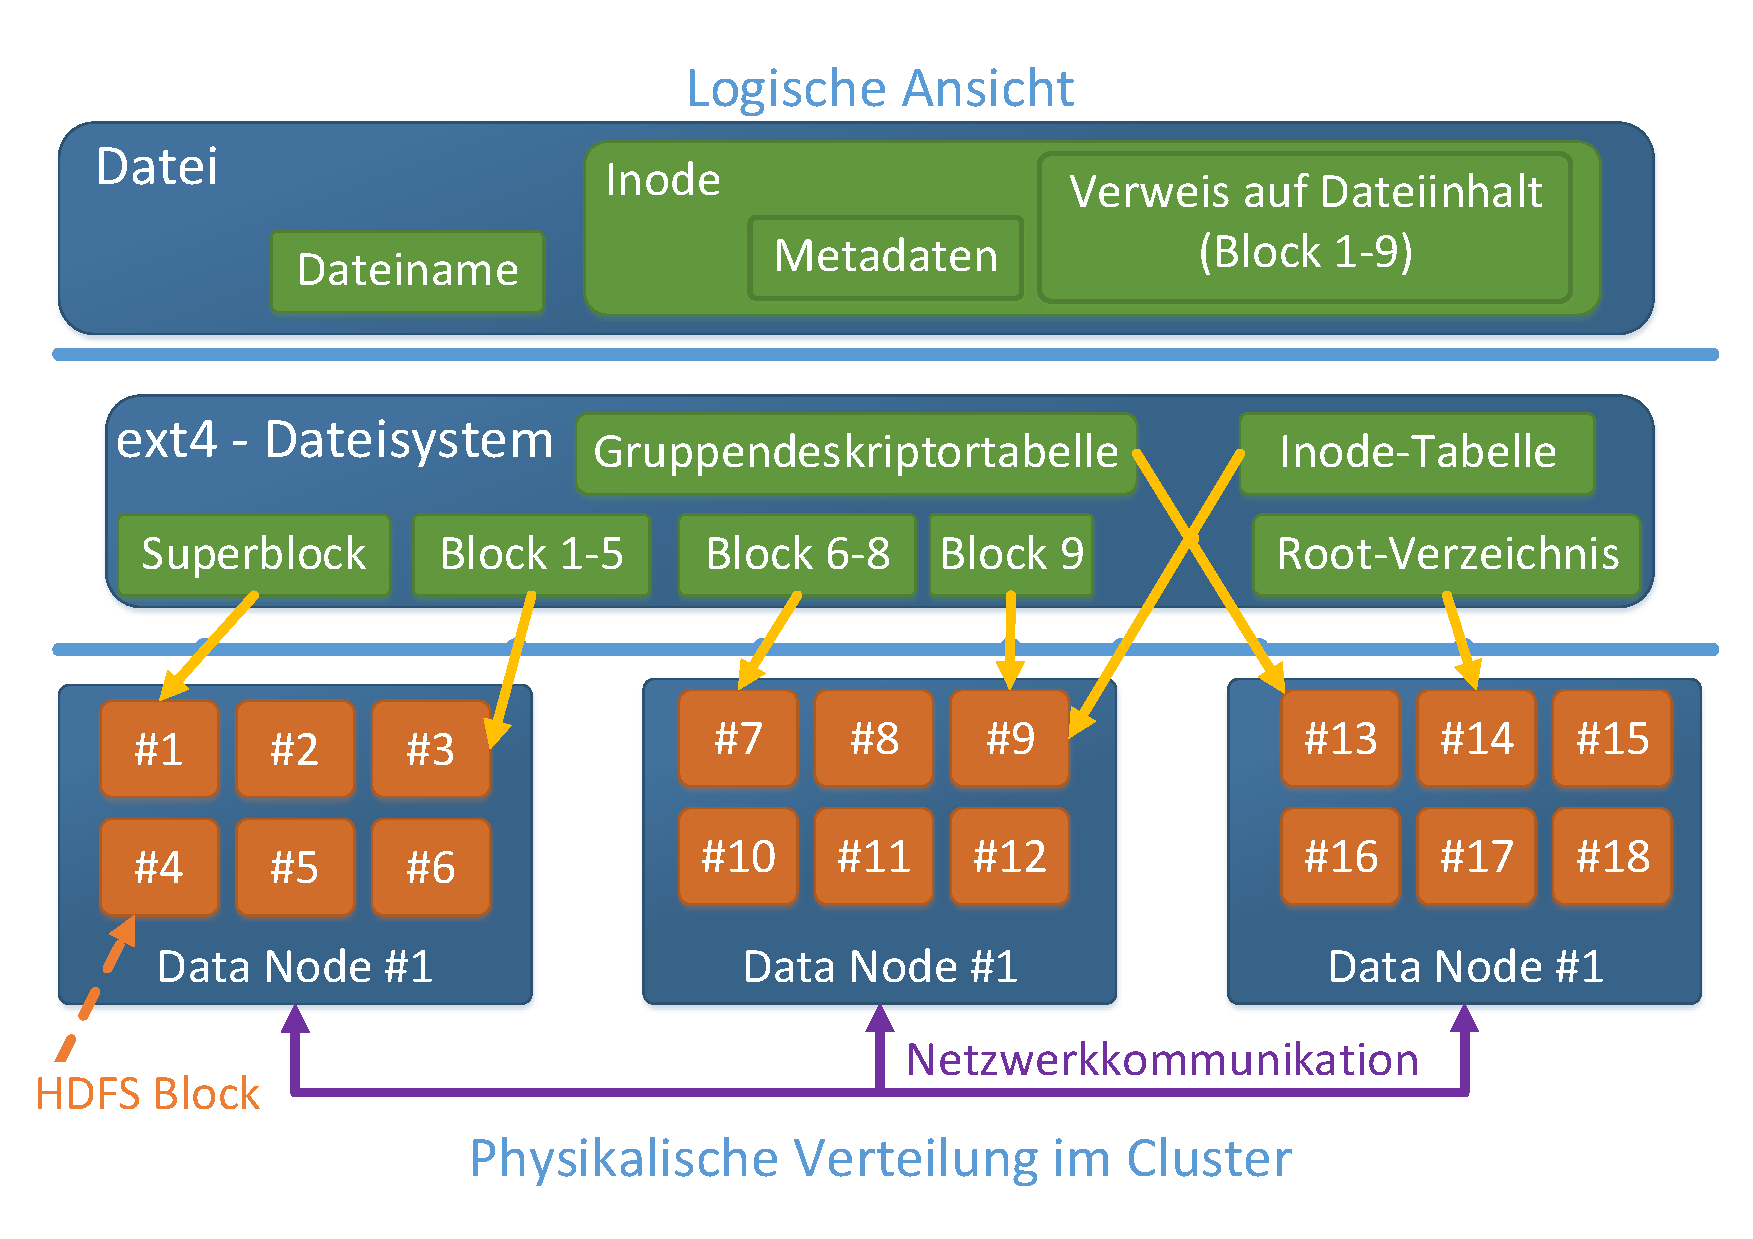
\includegraphics[width=\textwidth]{./resource/ext4_to_hdfs.pdf}
  \caption{Aufteilung der Daten des Datenträgerabbildes im Hadoop-Cluster}
  \label{fig:ext4_to_hdfs}
\end{figure}

\noindent
Das Abbild zeigt eine Datei, welche aus logischer Sicht einen Dateinamen, Metadaten (beispielsweise Zugriffsrechte) und einen Inhalt besitzt. Der Inhalt ist in 9 Blöcken zu jeweils 2048 Byte aufgeteilt.\footnote{Die Blockgröße wird hierbei vom Ext4-Dateisystem bestimmt und ist die kleinste allozierbare Einheit im Dateisystem. In der physikalischen Aufteilung im HDFS Dateisystem gibt es auch Blöcke, welche aber beispielsweise eine Größe von 128 MB aufweisen (orange in Abbildung \ref{fig:ext4_to_hdfs}).} Um nun den Inhalt aus dem ext4-Dateisystem einer Datei auszulesen. Wird zuerst der Superblock benötigt. Dieser enthält allgemeine Informationen zum Dateisystem. Darauf wird die Gruppendeskriptortabelle benötigt, um auf einzelne Blockgruppen zuzugreifen.\footnote{Das Dateisystem selbst in mehrere autarke Bereiche unterteilt, welche für sich genommen eigenständig Daten einer Teilmenge aller Dateien vorhalten. Dies sind sogenannten Blockgruppen.} Über eine Blockgruppe kann wiederum auf die Inode-Tabelle zugegriffen werden. Diese speichert die Metadaten einzelner Dateien als sogenannte Inodes ab. Ein konkreter Inode-Eintrag hält wiederum Verweise auf die konkreten Blöcke, welche den Dateiinhalt beschreiben. Der Dateiname selbst wiederum in den logisch übergeordneten Verzeichnissen gespeichert. Das oberste Verzeichnis, ist das Wurzelverzeichnis. Dieses enthält den Namen einer Datei und die Referenz zum Inode.\\

\noindent
Letztlich zeigt diese Struktur, dass selbst beim Auslesen einer kleinen Datei etliche Speicherstellen innerhalb des Dateisystems gelesen und interpretiert werden müssen. Angenommen, dass ein konkretes ext4-Dateisystem in einer 100 GB großen Partition gespeichert wird, so wir diese große Datei im HDFS-Dateisystem in 800 große Blöcke zu je 128 MB aufgeteilt und auf den einzelnen Knoten des Clusters gespeichert. Hierbei kann aber kein Einfluss darauf genommen werden, wo welche Blöcke mit welchem Inhalt gespeichert werden. Letztlich bedeutet dies wiederum, wenn in einem Apache Spark Executor zu Verarbeitung der Daten eine Datei des Knotens gelesen werden soll, müssen prinzipiell etlichen Datenbereiche von anderen Knoten angefordert werden. Und dadurch wird auf Netzwerkebene unnötig viel Last erzeugt. Letztlich gilt für das Prinzip der Datenlokalität, dass die einzelnen Blöcke im HDFS möglichst unabhängig von einander verarbeitet werden können. Diese Problematik trifft übrigens nicht nur bei Ext-Dateisystemfamilie auf sondern auch bei anderen Dateisystemen.\\

\noindent
Aus den oben genannten Gründen ist die direkte Speicherung kompletter Datenträger im HDFS nicht geeignet für die Analyse im Hadoop-Cluster.

\subsection{Variante 2 - Logische Dateien im HDFS speichern}
Die zweite Variante wäre das Beweismittel auf dem lokalen Analyserechner zu mounten und alle Dateien auf logischer Ebene direkt in das HDFS zu importieren. 
Damit wäre die gesamte Dateisystemstruktur aus dem Datenträgerabbild im HDFS abgelegt. Allerdings wäre File Carving beziehungsweise das Auffinden von gelöschten Dateien nicht mehr im Hadoop-Framework möglich, sofern nicht auch der das Datenträgerabbild selbst nochmals in das HDFS importiert wird.\\ 

\noindent
Interessanter an dieser Variante ist aber das Verhalten des HDFS bezüglich der Metadaten und der unterschiedlichen Dateigröße. Bei dem Importierten müsste darauf geachtet werden, dass alle Metadaten des lokalen Dateisystem im Datenträgerabbild unverändert in das HDFS kopiert werden. 
Welche Metadaten bereits im HDFS mit angelegt werden, zeigt Abbildung \ref{fig:hdfs_file_properties} anhand eines Ausschnitts aus der Web-Repräsentation eines HDFS.\\
\begin{figure}[ht]
  \centering
  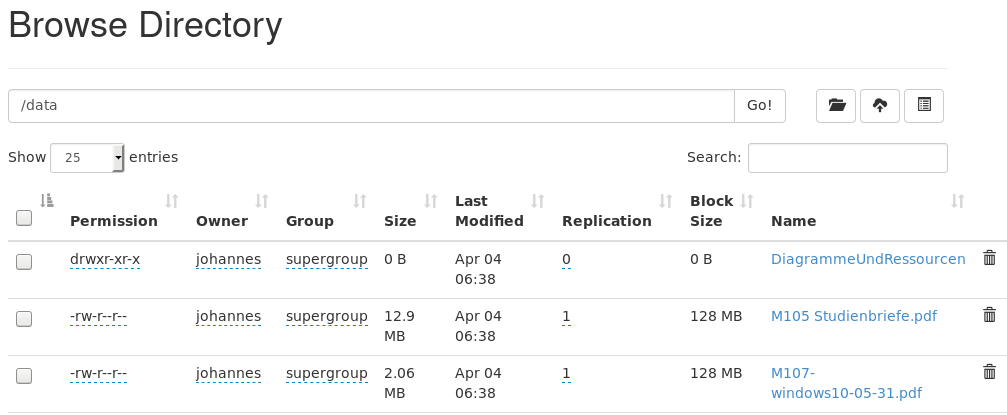
\includegraphics[width=\textwidth]{./resource/HDFS_FS_Example.png}
  \caption{HDFS - Dateieigenschaften}
  \label{fig:hdfs_file_properties}
\end{figure}

\noindent
Daraus ist ersichtlich, dass jede Datei entsprechende Dateirechte hat und einem Nutzer und einer Gruppe zugeordnet ist. Zusätzlich wird die Größe (nicht bei Verzeichnissen) und der Zeitstempel der letzten Änderung gespeichert. Die Anzahl der Replikationen und die Blockgröße sind spezifisch für das HDFS. Jede Datei kann auf einer unterschiedlichen Anzahl von Knoten repliziert sein. Die Standardkonfiguration definiert 3 Replikationen im realen Cluster, wobei Verzeichnisse nur logisch auf dem Name Node gehalten werden und damit auf keinem DataNode explizit repliziert werden. Auch die Blockgröße ist in der Standardkonfiguration auf 128 MB festgelegt. Wie im Grundlagenkapitel erwähnt, werden die Dateien in mehren Blöcken zu maximal 128 MB (konfigurationsabhängig) gespeichert und auch repliziert.\\ Bezogen auf klassische Dateisystem entspricht dies auch einem Block im ext4-Dateisystem oder einem Cluster im NTFS-Dateisystem (TODO: Quellenangabe!!! S.22 in M111). Es ist letztendlich die kleinste allozierbare Dateneinheit im Dateisystem. Dies bedeutet allerdings nicht, dass für jede Datei im HDFS auf den jeweiligen Date Nodes immer mindestens 128 MB Speicher belegt werden. Denn die reale Speicherbelegung auf dem Data Node beschränkt sich auch auf die reale Größe der Datei im lokalen Dateisystem des Data Nodes.\\

\noindent
Mit dem Befehl aus Listing \ref{lst:hdfs_put_command} können Dateien von einem lokalen Verzeichnis in das HDFS importiert werden. 
\begin{lstlisting}[label={lst:hdfs_put_command},caption= Befehl zum Speichern einer Datei im HDFS,captionpos=b,frame=single,style=customshell]
hdfs dfs -put test.pdf /test.pdf
\end{lstlisting}
Hierbei werden die ursprünglichen Metadaten der Datei nicht übernommen. So beschreibt der oben erwähnte Modifikationszeitstempel den Zeitpunkt, zu dem die Datei im HDFS das letzte Mal geändert wurde. Dies entspricht initial dem Import-Zeitpunkt. Auch werden Nutzer und Gruppenrechte nicht übernommen. Prinzipiell wäre es aber möglich die Metadaten aus dem lokalen Dateisystem mit in das HDFS zu übernehmen.\footnote{Hierzu kann dem \textit{put}-Befehl aus Listing \ref{lst:hdfs_put_command} der Parameter \textit{-p} mit übergeben werden.} Ratsam ist dies jedoch nicht, da gerade auch der Nutzer, die Gruppe und die dazugehörigen Zugriffsrechte in einem produktiven HDFS-Cluster verwendet werden, um Zugriffsbeschränkungen einzelner Nutzer und einzelner Programme umzusetzen.\\

\noindent
In der Theorie können noch weitere Metadaten gespeichert werden. Hierbei können erweiterte Dateiattribute beliebige Informationen über die Datei speichern. Mit nachfolgendenen Befehlen kann beispielsweise der originale Zeitstempel der Erstellung einer Datei hinzugefügt und ausgelesen werden. Hierbei kann der Name des Attributs und dessen Inhalt frei gewählt werden.
\begin{lstlisting}[label={lst:hdfs_fattr_command},caption= Befehl zum Hinzufügen und Auslesen von Metadaten,captionpos=b,frame=single,style=customshell]
# Create custom file attribute
hdfs dfs -setfattr -n user.ntfs.creationtime -v "2018-04-07T11:14:42,798583789+02:00" /test.pdf

# Read custom file attribute
hdfs dfs -getfattr -d -n user.ntfs.creationtime /test.pdf
\end{lstlisting}

\noindent
Mit dem obigen Befehl wäre es also prinzipiell möglich, Metadaten des ursprünglichen Dateisystems zu übernehmen. Allerdings müssen diese Metadaten zur Weiterverarbeitung zuerst für jede Datei im HDFS eingetragen werden.\\
Zusätzlich müssen beim Prozessieren der Daten mit Apache Spark die Metadaten auslesbar sein. Dieses Auslesen ist umständlich aber möglich.\footnote{Siehe Metadaten-Extraktion im Projekt \textit{foam-processing-spark} unter \url{https://github.com/jobusam/foam-processing-spark}.}\\ 
Letztlich ist es wohl aber auch ein Performance-Problem, denn diese Metadaten werden auf dem Namenode gespeichert.\footnote{Siehe \url{https://de.hortonworks.com/blog/hdfs-metadata-directories-explained/}, Stand 6.4.2018.} Somit müsste jeder Datanode diese Informationen wiederum explizit am Namenode anfragen.\\

\noindent
Das Fazit der Variante 2 lautet daher, dass die Dateimetadaten des originalen Datenträgerabbildes höchstens als erweiterte Attribute im HDFS abgelegt werden könnten. Beim Importieren müssten diese Metadaten bei jeder einzelnen Datei explizit nachgetragen werden. Pro Datei wäre dies nochmals ein eigener HDFS-Aufruf. Nicht zuletzt werden diese erweiterten Metadaten physikalisch im Namenode gespeichert. Dadurch benötigt der Namenode mehr Speicher. Viel schwerwiegender jedoch ist, dass die erweiterten Metadaten beim Prozessieren mit Spark angefordert werden müssten und somit der Namenode viel zu stark beansprucht werden würde.\\
Aus diesen Gründen ist die Variante 2 nicht akzeptabel. 

\noindent
TODO: weiterer Aspekt - performantes Prozessieren von vielen kleinen Dateien / bwz. Dateien unterschiedlicher Größe!!!\\

\subsection{Variante 3 - ZIP-File bzw. Hadoop Archive?}
Die Nachteile aus Variante 2 beziehen sich in erster Linie auf die Speicherung der Datei-Metadaten. Diese sollten nicht als erweiterte Dateiattribute im HDFS gespeichert werden, da sie sonst bei der Verarbeitung den Name Node im Hadoop Cluster überfordern könnten. Ein weiterer Nachteil wäre hierbei auch, dass das HDFS sehr gut mit großen Dateien umgehen kann, aber für kleine Dateien ( << 128 MB) nicht ausgelegt ist. Weil eben die Metadaten im Name Node gespeichert werden und generell der Ressourcenaufwand der Speicherung einer HDFS-Datei nicht im Verhältnis zu einer kleinen 1 kByte-Datei steht. Dies zeigt sich auch bei den Testdaten. Auf einem 10 GB großen Testdatenträgerabbild wurde ein Ubuntu-Linux installiert und einige Nutzeroperationen durchgeführt. Nachfolgende Abbildung zeigt die Anzahl der Dateien gruppiert nach deren Größe. Hier wird deutlich, dass es bei der Analyse von Datenträgern primär um das Verarbeiten sehr vieler und sehr kleiner Dateien geht. \\
TODO: Hadoop Sequence File. An sich nicht schlecht, allerdings müssen sequence files vorher lokal erstellt werden. Dann muss die Import-App auf dem Analyse-Rechner zuerst die Daten Laden umstrukturieren und wieder auf die lokale Platte schreiben, um sie dann letztendlich als Sequnce-File direkt hochladen zu können. Viel schwerwiegender ist jedoch, dass einmal erstelle Dateien im HDFS maximal um Daten am Dateiende erweitert werden können (Append-Mode).  Wenn ich jedoch zu den einzelnen Dateien weitere Metadaten während der Analyse ermittle, dann müssen diese ja auch in irgendeiner Art und Weise an die Sequence-Dateien angehangen werden. Diese wäre nicht sehr sinnvoll. 
Costum Forensic Format
Metadaten,Blockaufteilung,logische Sicherung\\
nachteil, carving muss vorher passieren...

Nachteil, wenn Metadaten (Hashes,File-Typen, etc...) hinzukommen müssten die Dateien neu berechnet werden...

\subsection{Variante 4 - Speicherung mit HBASE und HDFS}
Diese Variante beschreibt einen Ansatz, bei welchem die Metadaten und sehr kleine Dateien direkt in HBASE persistiert werden. Dateien größer 10 MB werden direkt im HDFS abgelegt und im jeweiligen Dateieintrag in HBASE verlinkt. Auch hier muss beim Import der Daten eine eigene Anwendung die Informationen aus dem Datenträgerabbild auslesen und entsprechend ihrer Struktur in HBASE und HDFS speichern. Das GitHub-Projekt \textit{foam-data-import} enthält diese Anwendung (siehe \url{https://github.com/jobusam/foam-data-import}).\\


Abbildung \ref{fig:data_import} skizziert die Datenaufbereitung und Speicherung in HBASE und im HDFS.\\
\begin{figure}[ht]
  \centering
  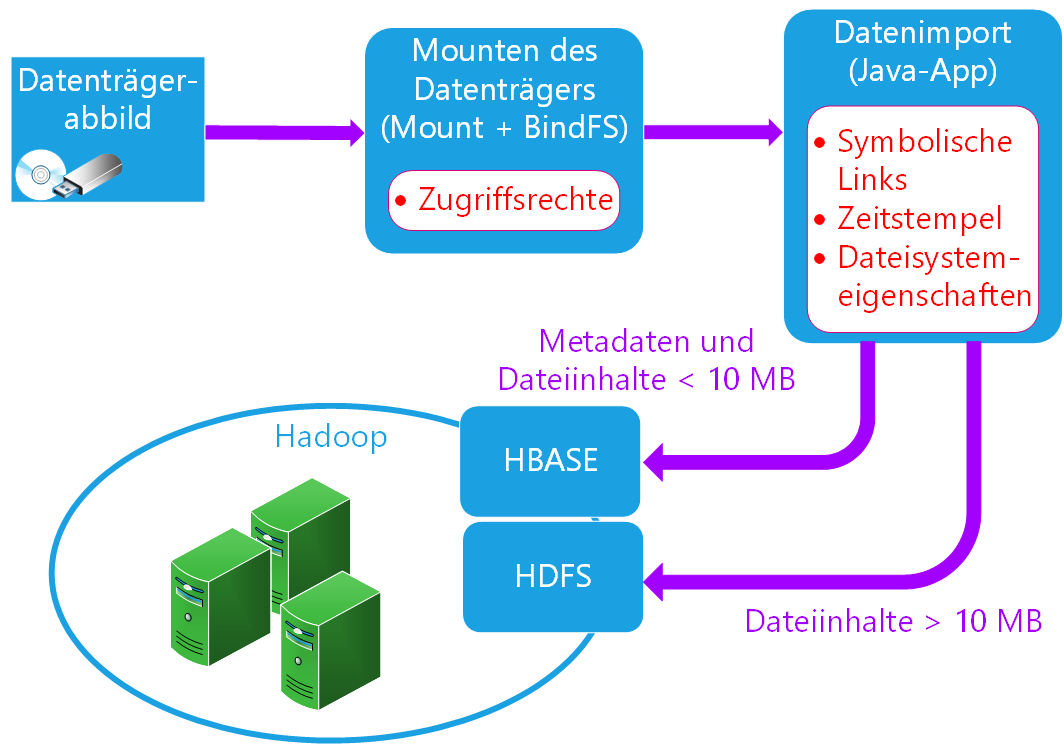
\includegraphics[width=\textwidth]{./resource/datenimport_hadoop.png}
  \caption{Datenimport in HBASE und HDFS}
  \label{fig:data_import}
\end{figure}

\subsubsection{Datenmodell}

Das Datenmodell beschreibt die Struktur der Metadaten und verdeutlicht den Informationsgehalt der forensischen Analyseplattform. 

\begin{table}[!ht]
\centering
\begin{tabular}{|l|l|p{8cm}|}\hline
\bfseries Spaltenfamilie & \bfseries Spaltenname & \bfseries Beschreibung
\csvreader[head to column names]{resource/hbase_datamodel.csv}{}
{\\\hline \columnfamily & \column & \description}\\\hline
\end{tabular}
\caption{Datenmodell in HBASE}
\label{tab:hbase_datamodel}
\end{table}

TODO: Datenimport mit unterschiedlicher Dateigröße aufzeigen.

%\noindent
%TODO: Siehe HBASE MOB (Medium-sized Object Binaries)
TODO: Fazit der vor und nachteile aller varianten, um zu zeigen wie variante 2 besser als 1 ist und variante 3 besser als 2 wäre und variante 4 die beste variante ist!
\section{Fachliche Probleme bei den Daten}

\subsection{Symbolische Links}
Es gibt einige Hürden beim Importieren der Datenträger in das HDFS. Wie bereits erwähnt werden die Daten auf logischer Dateiebene in das Hadoop-System importiert. Hierbei müssen spezielle Dateitypen berücksichtigt werden. Ein Beispiel ist die Verarbeitung von symbolischen Links, welche gerade unter Linux-basierten Betriebssystemen beziehungsweise in der EXT-Dateisystemfamilie auftreten können. Denn wenn symbolische Links in einem Dateisystem gespeichert werden und letzteres im Analysesystem gemountet wird, so können diese Links auch auf Dateien außerhalb des Dateisystems verweisen. Denn letztlich interpretiert das Betriebssystem diese symbolischen Links. Bei der forensischen Analyse könnte diese aber zu schwerwiegenden Fehlern der Analyseergebnisse führen, wenn beispielsweise Inhalte des Analyserechners verarbeitet werden, welche ursprünglich nicht auf dem Asservat vorhanden waren. Daher muss beim Import auf geprüft werden, ob die Datei einem symbolischen Link entspricht. Ist dies der Fall darf, der symbolische Link nicht interpretiert werden. 

\subsection{Zugriffsrechte}
Ein weiterer Aspekt ist die Beschränkung der Dateizugriffe auf Basis der vorgegebenen Zugriffsrechte. Angenommen es wird ein Datenträgerabbild auf einem Analysesystem gemountet.
Dann kann dies im Normalfall nur mit Root-Rechten durchgeführt werden. 
Der forensische Analyse benötigt also zumindest auf seinem Analyse-Rechner 
privilegierte Ausführungsrechte.\\
Beim Import von Dateien auf eben diesem gemounteten Dateisystem des Datenträgerabbildes sind jedoch die Dateizugriffsrechte weitaus interessanter. Denn das Analyse-Betriebssystem berücksichtigt diese Zugriffsrechte. Während diese Problematik beispielsweise bei NTFS-Dateisystemen eine untergeordnete Rolle spielt, so werden hingegen bei EXT-Dateisystemen die Unix-Dateirechte gespeichert und auch auf dem Analysesystem interpretiert. 
Daher kann der Nutzer und dessen ausgeführte Programme, welche die Daten aus dem Dateisystem auslesen, nicht in allen Fällen auf alle Dateien zugreifen.\\

\noindent
Die einfachste Möglichkeit um die Problematik der Zugriffsrechte zu umgehen, wäre das Ausführen der Datenimport-Applikation mit Root-Rechten. Andererseits sollte die Datenimport-Applikation aber nicht mit Root-Rechten ausgestattet werden, da dies zu Sicherheitslücken und unvorhergesehenen Rechteausweitungen im Fehlerfall führen könnte. Darüber hinaus kann bei einem Fehlverhalten der Anwendung das Analysesystem beschädigt werden. \\
Letztlich braucht die Anwendung zum Datenimport nur die Berechtigungen zum Lesen von Dateien mit Root-Rechten. Dies würde dem \textit{Need-to-know-Prinzip} genügen.\\
%(TODO: verweis auf s. 42 M106)

\noindent
Eigentlich müsste beim Mounten des Dateisystems dem Betriebssystem mitgeteilt werden können, dass die Dateirechte des gemounteten Dateisystems ignoriert werden sollen. Diese Option ist aber nicht möglich\footnote{Zumindest konnte keine funktionierende Variante gefunden werden (siehe Man-Page des Mount-Befehls.}.\\
Eine weitere Alternative wäre die Möglichkeit mit Access Control Lists (ACL) zu arbeiten und dem nichtprivilegiertem Nutzer Rechte zum Lesen der Dateien zu geben. Oder umgekehrt alle Dateien dem nichtprivilegierten Nutzer zuzordnen, welcher wiederum den Datenimport startet.
Hierzu müsste die Datenträgerkopie schreibend gemountet werden, damit die Rechte jeder Datei angepasst werden können. Dies würde wiederum dazu führen, dass das Datenträgerabbild als sichergestelltes Asservat geändert werden würde. 
Daher ist diese Lösung auch nicht geeignet.\\

\noindent
Eine weitere Alternative ist die Nutzung von Posix Capabilities\footnote{Siehe Manpages mit folgendem Befehl: \textit{ man 7 capabilities}.}.
Dies scheint unter CentOS/Fedora wohl die beste Variante zu sein. Zum Lesenden Zugriff auf Dateien müsste die Posix Capability \textit{CAP\_DAC\_READ\_SEARCH} gesetzt werden.\\
Mit nachfolgenden Kommando könnte diese Capability dem Analyseprogramm gesetzt werden.
Damit könnte dann auch ein nicht-privilegierte Nutzer lesenden Zugriff auf privilegierte Dateien erhalten.\\ 

\begin{lstlisting}[label={lst:pos_cap_command},caption= Befehl zum Setzen von Posix Capabilities,captionpos=b,frame=single,style=customshell]
setcap CAP_DAC_READ_SEARCH /bin/forensic_import
\end{lstlisting}
% Mit oder ohne + eip???
%setcap CAP\_DAC\_READ\_SEARCH+eip /bin/ping

\noindent
Allerdings funktioniert diese Art hauptsächlich bei Binärprogrammen aber nicht bei Shell-Skripten oder Java-Anwendungen. Ein ähnliche Alternative zu Posix Capabilities ist das Setzen des SUID-Bits als Unix-Dateirecht für die Programmdatei. Aber auch gilt wieder, dass dies für Binärprogramme funktioniert aber nicht für interpretierte Skripte oder Java-Anwendungen, welche wiederum in der Java Virtual Machine laufen.
%Setzen des Flags
%chmod u-s /bin/ping

Die Nutzung von SELINUX empfiehlt sich hier auch nicht. SELINUX ist eine Erweiterung des Linux-Kernels um detaillierte Zugriffskontrollen zu setzen. Diese Erweiterung ermöglicht eine detaillierte Definition, welche Anwendung oder Nutzer auf einzelne Dateien zugreifen dürfen. Allerdings werden auch unter SELINUX immer zuerst die Unix-Dateirechte und zusätzlich die in SELINUX definierten Zugriffskontrollen geprüft. Daher kann auch mit SELINUX das Problem nicht behoben werden.\\

\noindent
Zuletzt gibt es noch eine Variante, welche die Problematik mit den Dateirechten lösen kann. 
Mit dem Projekt \textit{bindfs}\footnote{Siehe \url{https://bindfs.org/}.} können unter Linux Dateisystemverzeichnisse neu gemountet werden und ihre Zugriffsrechte verändert werden. Der nachfolgende Befehl mountet das existierende Verzeichnis mit den enthaltenden Dateien in einem neuen Verzeichnis und setzt beispielsweise bei jeder Datei die aktuelle ID des Nutzers als Datei-Owner und Group. 
\begin{lstlisting}[label={lst:bindfs_command},caption= Nutzung von Bindfs zum Ändern von Dateirechten,captionpos=b,frame=single,style=customshell]
sudo bindfs -u $(id -u) -g $(id -g) src_dir/ target_dir/
\end{lstlisting}
Der Befehl selbst benötigt Root-Rechte. Jedoch kann der Nutzer danach alle Dateien des Zielverzeichnisses lesen. Der einzige Nachteil an dieser Lösung ist, dass der Besitzer und die Gruppe jeder einzelnen Datei nun der Nutzer des Analysesystems ist.\\
Dieser Nachteil muss zukünftig behoben werden, damit die forensische Analyseplattform auch die Besitzer und Gruppen einer Datei korrekt auswerten kann.
%Im Anhang beschreiben, wie bindfs gebaut werden kann.